\documentclass[twoside]{article}

% Packages required by doxygen
\usepackage{calc}
\usepackage{doxygen}
\usepackage{graphicx}
\usepackage[utf8]{inputenc}
\usepackage{makeidx}
\usepackage{multicol}
\usepackage{multirow}
\usepackage{textcomp}
\usepackage[table]{xcolor}

% Font selection
\usepackage[T1]{fontenc}
\usepackage{mathptmx}
\usepackage[scaled=.90]{helvet}
\usepackage{courier}
\usepackage{amssymb}
\usepackage{sectsty}
\renewcommand{\familydefault}{\sfdefault}
\allsectionsfont{%
  \fontseries{bc}\selectfont%
  \color{darkgray}%
}
\renewcommand{\DoxyLabelFont}{%
  \fontseries{bc}\selectfont%
  \color{darkgray}%
}

% Page & text layout
\usepackage{geometry}
\geometry{%
  letterpaper,%
  top=2.5cm,%
  bottom=2.5cm,%
  left=2.5cm,%
  right=2.5cm%
}
\tolerance=750
\hfuzz=15pt
\hbadness=750
\setlength{\emergencystretch}{15pt}
\setlength{\parindent}{0cm}
\setlength{\parskip}{0.2cm}
\makeatletter
\renewcommand{\paragraph}{%
  \@startsection{paragraph}{4}{0ex}{-1.0ex}{1.0ex}{%
    \normalfont\normalsize\bfseries\SS@parafont%
  }%
}
\renewcommand{\subparagraph}{%
  \@startsection{subparagraph}{5}{0ex}{-1.0ex}{1.0ex}{%
    \normalfont\normalsize\bfseries\SS@subparafont%
  }%
}
\makeatother

% Headers & footers
\usepackage{fancyhdr}
\pagestyle{fancyplain}
\fancyhead[LE]{\fancyplain{}{\bfseries\thepage}}
\fancyhead[CE]{\fancyplain{}{}}
\fancyhead[RE]{\fancyplain{}{\bfseries\leftmark}}
\fancyhead[LO]{\fancyplain{}{\bfseries\rightmark}}
\fancyhead[CO]{\fancyplain{}{}}
\fancyhead[RO]{\fancyplain{}{\bfseries\thepage}}
\fancyfoot[LE]{\fancyplain{}{}}
\fancyfoot[CE]{\fancyplain{}{}}
\fancyfoot[RE]{\fancyplain{}{\bfseries\scriptsize Generated on Sun Jan 25 2015 10\-:33\-:32 for I\-M\-U Monitor by Doxygen }}
\fancyfoot[LO]{\fancyplain{}{\bfseries\scriptsize Generated on Sun Jan 25 2015 10\-:33\-:32 for I\-M\-U Monitor by Doxygen }}
\fancyfoot[CO]{\fancyplain{}{}}
\fancyfoot[RO]{\fancyplain{}{}}
\renewcommand{\footrulewidth}{0.4pt}
\renewcommand{\sectionmark}[1]{%
  \markright{\thesection\ #1}%
}

% Indices & bibliography
\usepackage{natbib}
\usepackage[titles]{tocloft}
\setcounter{tocdepth}{3}
\setcounter{secnumdepth}{5}
\makeindex

% Hyperlinks (required, but should be loaded last)
\usepackage{ifpdf}
\ifpdf
  \usepackage[pdftex,pagebackref=true]{hyperref}
\else
  \usepackage[ps2pdf,pagebackref=true]{hyperref}
\fi
\hypersetup{%
  colorlinks=true,%
  linkcolor=blue,%
  citecolor=blue,%
  unicode%
}

% Custom commands
\newcommand{\clearemptydoublepage}{%
  \newpage{\pagestyle{empty}\cleardoublepage}%
}


%===== C O N T E N T S =====

\begin{document}

% Titlepage & ToC
\hypersetup{pageanchor=false}
\pagenumbering{roman}
\begin{titlepage}
\vspace*{7cm}
\begin{center}%
{\Large I\-M\-U Monitor }\\
\vspace*{1cm}
{\large Generated by Doxygen 1.8.6}\\
\vspace*{0.5cm}
{\small Sun Jan 25 2015 10:33:32}\\
\end{center}
\end{titlepage}
\tableofcontents
\pagenumbering{arabic}
\hypersetup{pageanchor=true}

%--- Begin generated contents ---
\section{I\-M\-U Monitor}
\label{index}\hypertarget{index}{}\begin{DoxyAuthor}{Author}
Sebastián Sepúlveda 
\end{DoxyAuthor}
\begin{DoxyDate}{Date}
March 25, 2014 
\end{DoxyDate}
\begin{DoxyVersion}{Version}
0.\-9
\end{DoxyVersion}
\subsection*{Description}
\section{Hierarchical Index}
\subsection{Class Hierarchy}
This inheritance list is sorted roughly, but not completely, alphabetically\-:\begin{DoxyCompactList}
\item \contentsline{section}{activity\-Detection.\-Activity\-Detection}{\pageref{classactivity_detection_1_1_activity_detection}}{}
\item \contentsline{section}{csv\-Export.\-C\-S\-V\-Export}{\pageref{classcsv_export_1_1_c_s_v_export}}{}
\item \contentsline{section}{fall\-Detection.\-Fall\-Detection}{\pageref{classfall_detection_1_1_fall_detection}}{}
\item \contentsline{section}{imu.\-I\-M\-U}{\pageref{classimu_1_1_i_m_u}}{}
\item \contentsline{section}{log.\-Log}{\pageref{classlog_1_1_log}}{}
\item object\begin{DoxyCompactList}
\item \contentsline{section}{gui.\-Ui\-\_\-\-Main\-Window}{\pageref{classgui_1_1_ui___main_window}}{}
\end{DoxyCompactList}
\item \contentsline{section}{posture.\-Posture}{\pageref{classposture_1_1_posture}}{}
\item Q\-Main\-Window\begin{DoxyCompactList}
\item \contentsline{section}{main.\-Main\-Window}{\pageref{classmain_1_1_main_window}}{}
\end{DoxyCompactList}
\item Q\-Thread\begin{DoxyCompactList}
\item \contentsline{section}{base\-Thread.\-Base\-Thread}{\pageref{classbase_thread_1_1_base_thread}}{}
\begin{DoxyCompactList}
\item \contentsline{section}{cube.\-Cube}{\pageref{classcube_1_1_cube}}{}
\item \contentsline{section}{serial\-Thread.\-Serial\-Thread}{\pageref{classserial_thread_1_1_serial_thread}}{}
\item \contentsline{section}{serial\-Thread\-\_\-mutiprocessing.\-Serial\-Thread}{\pageref{classserial_thread__mutiprocessing_1_1_serial_thread}}{}
\end{DoxyCompactList}
\end{DoxyCompactList}
\item \contentsline{section}{sensor\-Fusion.\-Sensor\-Fusion}{\pageref{classsensor_fusion_1_1_sensor_fusion}}{}
\end{DoxyCompactList}

\section{Class Index}
\subsection{Class List}
Here are the classes, structs, unions and interfaces with brief descriptions\-:\begin{DoxyCompactList}
\item\contentsline{section}{\hyperlink{classactivity_detection_1_1_activity_detection}{activity\-Detection.\-Activity\-Detection} \\*Estimates the energy consumption (Kcal) by second }{\pageref{classactivity_detection_1_1_activity_detection}}{}
\item\contentsline{section}{\hyperlink{classbase_thread_1_1_base_thread}{base\-Thread.\-Base\-Thread} \\*Defines basic methods for dealing with Qt Threads and all Threads }{\pageref{classbase_thread_1_1_base_thread}}{}
\item\contentsline{section}{\hyperlink{classcsv_export_1_1_c_s_v_export}{csv\-Export.\-C\-S\-V\-Export} \\*Export data in C\-S\-V format }{\pageref{classcsv_export_1_1_c_s_v_export}}{}
\item\contentsline{section}{\hyperlink{classcube_1_1_cube}{cube.\-Cube} \\*Displays the orientation as a 3\-D cube }{\pageref{classcube_1_1_cube}}{}
\item\contentsline{section}{\hyperlink{classfall_detection_1_1_fall_detection}{fall\-Detection.\-Fall\-Detection} \\*Detects fall from the accelerometer data }{\pageref{classfall_detection_1_1_fall_detection}}{}
\item\contentsline{section}{\hyperlink{classimu_1_1_i_m_u}{imu.\-I\-M\-U} \\*\hyperlink{classimu_1_1_i_m_u}{I\-M\-U} values for scales and data structure in the C\-S\-V data received }{\pageref{classimu_1_1_i_m_u}}{}
\item\contentsline{section}{\hyperlink{classlog_1_1_log}{log.\-Log} \\*General logging for debugging }{\pageref{classlog_1_1_log}}{}
\item\contentsline{section}{\hyperlink{classmain_1_1_main_window}{main.\-Main\-Window} \\*Managing and plotting adquired data }{\pageref{classmain_1_1_main_window}}{}
\item\contentsline{section}{\hyperlink{classposture_1_1_posture}{posture.\-Posture} \\*\hyperlink{classposture_1_1_posture}{Posture} estimation based on accelerometer used as a compensated tilt sensor }{\pageref{classposture_1_1_posture}}{}
\item\contentsline{section}{\hyperlink{classsensor_fusion_1_1_sensor_fusion}{sensor\-Fusion.\-Sensor\-Fusion} \\*Algorithms and functions for 9\-D\-O\-F fusion }{\pageref{classsensor_fusion_1_1_sensor_fusion}}{}
\item\contentsline{section}{\hyperlink{classserial_thread_1_1_serial_thread}{serial\-Thread.\-Serial\-Thread} \\*Obtain and scale serial data in a thread }{\pageref{classserial_thread_1_1_serial_thread}}{}
\item\contentsline{section}{\hyperlink{classserial_thread__mutiprocessing_1_1_serial_thread}{serial\-Thread\-\_\-mutiprocessing.\-Serial\-Thread} \\*Obtain and scale serial data in a thread }{\pageref{classserial_thread__mutiprocessing_1_1_serial_thread}}{}
\item\contentsline{section}{\hyperlink{classgui_1_1_ui___main_window}{gui.\-Ui\-\_\-\-Main\-Window} }{\pageref{classgui_1_1_ui___main_window}}{}
\end{DoxyCompactList}

\section{Class Documentation}
\hypertarget{classcsv_export_1_1_c_s_v_export}{\subsection{csv\-Export.\-C\-S\-V\-Export Class Reference}
\label{classcsv_export_1_1_c_s_v_export}\index{csv\-Export.\-C\-S\-V\-Export@{csv\-Export.\-C\-S\-V\-Export}}
}


Export data in C\-S\-V format.  


\subsubsection*{Public Member Functions}
\begin{DoxyCompactItemize}
\item 
def \hyperlink{classcsv_export_1_1_c_s_v_export_ac878a5b6f1169cc205547656c00e64d5}{\-\_\-\-\_\-init\-\_\-\-\_\-}
\begin{DoxyCompactList}\small\item\em Constructor. \end{DoxyCompactList}\item 
def \hyperlink{classcsv_export_1_1_c_s_v_export_a5b5e890619df75ddc137184f59036d09}{csv\-Write}
\begin{DoxyCompactList}\small\item\em Writes a new line of data. \end{DoxyCompactList}\end{DoxyCompactItemize}
\subsubsection*{Public Attributes}
\begin{DoxyCompactItemize}
\item 
\hypertarget{classcsv_export_1_1_c_s_v_export_ae6d8f4d693e9421b2e317def0815719e}{{\bfseries C\-S\-V}}\label{classcsv_export_1_1_c_s_v_export_ae6d8f4d693e9421b2e317def0815719e}

\item 
\hypertarget{classcsv_export_1_1_c_s_v_export_a8b226cc63eecae0145db1a0c6975c870}{{\bfseries t0}}\label{classcsv_export_1_1_c_s_v_export_a8b226cc63eecae0145db1a0c6975c870}

\end{DoxyCompactItemize}


\subsubsection{Detailed Description}
Export data in C\-S\-V format. 

Export data using date and time as name for the file, avoiding overwriting data in differents adquisitions.

It also registers in the first colummn the elapsed since the first adquisition

\begin{DoxyNote}{Note}
The data is stored in a \char`\"{}data\char`\"{} folder (muest be created first) 
\end{DoxyNote}


\subsubsection{Constructor \& Destructor Documentation}
\hypertarget{classcsv_export_1_1_c_s_v_export_ac878a5b6f1169cc205547656c00e64d5}{\index{csv\-Export\-::\-C\-S\-V\-Export@{csv\-Export\-::\-C\-S\-V\-Export}!\-\_\-\-\_\-init\-\_\-\-\_\-@{\-\_\-\-\_\-init\-\_\-\-\_\-}}
\index{\-\_\-\-\_\-init\-\_\-\-\_\-@{\-\_\-\-\_\-init\-\_\-\-\_\-}!csvExport::CSVExport@{csv\-Export\-::\-C\-S\-V\-Export}}
\paragraph[{\-\_\-\-\_\-init\-\_\-\-\_\-}]{\setlength{\rightskip}{0pt plus 5cm}def csv\-Export.\-C\-S\-V\-Export.\-\_\-\-\_\-init\-\_\-\-\_\- (
\begin{DoxyParamCaption}
\item[{}]{self}
\end{DoxyParamCaption}
)}}\label{classcsv_export_1_1_c_s_v_export_ac878a5b6f1169cc205547656c00e64d5}


Constructor. 

Gets time to create the filename and instanciate the start of the adquisition \begin{DoxyNote}{Note}
The filename format is Year-\/\-Moth-\/\-Day\-\_\-\-Hours-\/minutes-\/seconds.\-csv 
\end{DoxyNote}


\subsubsection{Member Function Documentation}
\hypertarget{classcsv_export_1_1_c_s_v_export_a5b5e890619df75ddc137184f59036d09}{\index{csv\-Export\-::\-C\-S\-V\-Export@{csv\-Export\-::\-C\-S\-V\-Export}!csv\-Write@{csv\-Write}}
\index{csv\-Write@{csv\-Write}!csvExport::CSVExport@{csv\-Export\-::\-C\-S\-V\-Export}}
\paragraph[{csv\-Write}]{\setlength{\rightskip}{0pt plus 5cm}def csv\-Export.\-C\-S\-V\-Export.\-csv\-Write (
\begin{DoxyParamCaption}
\item[{}]{self, }
\item[{}]{txt}
\end{DoxyParamCaption}
)}}\label{classcsv_export_1_1_c_s_v_export_a5b5e890619df75ddc137184f59036d09}


Writes a new line of data. 


\begin{DoxyParams}{Parameters}
{\em self} & The object pointer \\
\hline
{\em txt} & The data to export \\
\hline
\end{DoxyParams}


The documentation for this class was generated from the following file\-:\begin{DoxyCompactItemize}
\item 
I\-M\-U\-Graph/csv\-Export.\-py\end{DoxyCompactItemize}

\hypertarget{classserver_1_1_imu}{\subsection{server.\-Imu Class Reference}
\label{classserver_1_1_imu}\index{server.\-Imu@{server.\-Imu}}
}


I\-M\-U class to access data.  




Inheritance diagram for server.\-Imu\-:
\nopagebreak
\begin{figure}[H]
\begin{center}
\leavevmode
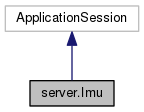
\includegraphics[width=180pt]{classserver_1_1_imu__inherit__graph}
\end{center}
\end{figure}


Collaboration diagram for server.\-Imu\-:
\nopagebreak
\begin{figure}[H]
\begin{center}
\leavevmode
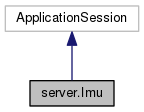
\includegraphics[width=180pt]{classserver_1_1_imu__coll__graph}
\end{center}
\end{figure}
\subsubsection*{Public Member Functions}
\begin{DoxyCompactItemize}
\item 
def \hyperlink{classserver_1_1_imu_af62e172c10fa382486a07c094adeaade}{on\-Join}
\begin{DoxyCompactList}\small\item\em on\-Join event (server connected) \end{DoxyCompactList}\item 
def \hyperlink{classserver_1_1_imu_a686e73f3cefe0b4a88623c68c3c49b2b}{on\-Leave}
\begin{DoxyCompactList}\small\item\em on\-Leave event (server disconnected) \end{DoxyCompactList}\item 
def \hyperlink{classserver_1_1_imu_a4bfc4c8632b7769ca36a773c0b39df92}{test}
\begin{DoxyCompactList}\small\item\em test function \end{DoxyCompactList}\item 
def \hyperlink{classserver_1_1_imu_ae090cee2a3aee7b1d9877357610b437c}{detect\-Imu}
\begin{DoxyCompactList}\small\item\em Detects the number of connected I\-M\-Us. \end{DoxyCompactList}\item 
def \hyperlink{classserver_1_1_imu_af407376e859abff47424fc4c2da7ea91}{set\-File\-Name}
\begin{DoxyCompactList}\small\item\em Sets filename for the C\-S\-V export. \end{DoxyCompactList}\item 
def \hyperlink{classserver_1_1_imu_af7b1a72e0d05b31931b955c294f1833e}{get\-File\-Name}
\begin{DoxyCompactList}\small\item\em Gets filename of the current C\-S\-V export. \end{DoxyCompactList}\item 
def \hyperlink{classserver_1_1_imu_a6b47186b53a976f9f851fc3b5c86e9cd}{start\-Imu}
\begin{DoxyCompactList}\small\item\em Starts adquisition. \end{DoxyCompactList}\item 
def \hyperlink{classserver_1_1_imu_a5d7f85a7405e74aced2c68294dafd485}{stopt\-Imu}
\begin{DoxyCompactList}\small\item\em Stops adquisition. \end{DoxyCompactList}\item 
def \hyperlink{classserver_1_1_imu_a3d15181eb786a459ed006e97fcf2c7c0}{get\-Imu\-Data}
\begin{DoxyCompactList}\small\item\em Get data. \end{DoxyCompactList}\end{DoxyCompactItemize}
\subsubsection*{Public Attributes}
\begin{DoxyCompactItemize}
\item 
\hypertarget{classserver_1_1_imu_af9ff83e11bf2dc2d3f2040de255ff270}{{\bfseries app}}\label{classserver_1_1_imu_af9ff83e11bf2dc2d3f2040de255ff270}

\end{DoxyCompactItemize}


\subsubsection{Detailed Description}
I\-M\-U class to access data. 

Defines callbacks and register events for W\-A\-M\-P server 
\begin{DoxyParams}{Parameters}
{\em Application\-Session} & W\-A\-M\-P instance \\
\hline
\end{DoxyParams}


\subsubsection{Member Function Documentation}
\hypertarget{classserver_1_1_imu_ae090cee2a3aee7b1d9877357610b437c}{\index{server\-::\-Imu@{server\-::\-Imu}!detect\-Imu@{detect\-Imu}}
\index{detect\-Imu@{detect\-Imu}!server::Imu@{server\-::\-Imu}}
\paragraph[{detect\-Imu}]{\setlength{\rightskip}{0pt plus 5cm}def server.\-Imu.\-detect\-Imu (
\begin{DoxyParamCaption}
\item[{}]{self, }
\item[{}]{arg = {\ttfamily None}}
\end{DoxyParamCaption}
)}}\label{classserver_1_1_imu_ae090cee2a3aee7b1d9877357610b437c}


Detects the number of connected I\-M\-Us. 


\begin{DoxyParams}{Parameters}
{\em self} & The object pointer. \\
\hline
{\em arg} & Expected data from the Web\-Socket \\
\hline
\end{DoxyParams}
\begin{DoxyReturn}{Returns}
number of I\-M\-Us detected 
\end{DoxyReturn}
\hypertarget{classserver_1_1_imu_af7b1a72e0d05b31931b955c294f1833e}{\index{server\-::\-Imu@{server\-::\-Imu}!get\-File\-Name@{get\-File\-Name}}
\index{get\-File\-Name@{get\-File\-Name}!server::Imu@{server\-::\-Imu}}
\paragraph[{get\-File\-Name}]{\setlength{\rightskip}{0pt plus 5cm}def server.\-Imu.\-get\-File\-Name (
\begin{DoxyParamCaption}
\item[{}]{self, }
\item[{}]{arg = {\ttfamily None}}
\end{DoxyParamCaption}
)}}\label{classserver_1_1_imu_af7b1a72e0d05b31931b955c294f1833e}


Gets filename of the current C\-S\-V export. 


\begin{DoxyParams}{Parameters}
{\em self} & The object pointer. \\
\hline
{\em arg} & Expected data from the Web\-Socket \\
\hline
\end{DoxyParams}
\begin{DoxyReturn}{Returns}
file name 
\end{DoxyReturn}
\hypertarget{classserver_1_1_imu_a3d15181eb786a459ed006e97fcf2c7c0}{\index{server\-::\-Imu@{server\-::\-Imu}!get\-Imu\-Data@{get\-Imu\-Data}}
\index{get\-Imu\-Data@{get\-Imu\-Data}!server::Imu@{server\-::\-Imu}}
\paragraph[{get\-Imu\-Data}]{\setlength{\rightskip}{0pt plus 5cm}def server.\-Imu.\-get\-Imu\-Data (
\begin{DoxyParamCaption}
\item[{}]{self, }
\item[{}]{arg = {\ttfamily None}}
\end{DoxyParamCaption}
)}}\label{classserver_1_1_imu_a3d15181eb786a459ed006e97fcf2c7c0}


Get data. 

Gets the current data from the current enabled sensor 
\begin{DoxyParams}{Parameters}
{\em self} & The object pointer. \\
\hline
{\em arg} & Expected data from the Web\-Socket \\
\hline
\end{DoxyParams}
\begin{DoxyReturn}{Returns}
sensor data 
\end{DoxyReturn}
\hypertarget{classserver_1_1_imu_af62e172c10fa382486a07c094adeaade}{\index{server\-::\-Imu@{server\-::\-Imu}!on\-Join@{on\-Join}}
\index{on\-Join@{on\-Join}!server::Imu@{server\-::\-Imu}}
\paragraph[{on\-Join}]{\setlength{\rightskip}{0pt plus 5cm}def server.\-Imu.\-on\-Join (
\begin{DoxyParamCaption}
\item[{}]{self, }
\item[{}]{details}
\end{DoxyParamCaption}
)}}\label{classserver_1_1_imu_af62e172c10fa382486a07c094adeaade}


on\-Join event (server connected) 

Starts the Main\-Process when server starts, initing the communication thread with the I\-M\-U 
\begin{DoxyParams}{Parameters}
{\em self} & The object pointer. \\
\hline
{\em details} & W\-A\-M\-P data \\
\hline
\end{DoxyParams}
\hypertarget{classserver_1_1_imu_a686e73f3cefe0b4a88623c68c3c49b2b}{\index{server\-::\-Imu@{server\-::\-Imu}!on\-Leave@{on\-Leave}}
\index{on\-Leave@{on\-Leave}!server::Imu@{server\-::\-Imu}}
\paragraph[{on\-Leave}]{\setlength{\rightskip}{0pt plus 5cm}def server.\-Imu.\-on\-Leave (
\begin{DoxyParamCaption}
\item[{}]{self, }
\item[{}]{details}
\end{DoxyParamCaption}
)}}\label{classserver_1_1_imu_a686e73f3cefe0b4a88623c68c3c49b2b}


on\-Leave event (server disconnected) 

Stops the Main\-Process when server stops. 
\begin{DoxyParams}{Parameters}
{\em self} & The object pointer. \\
\hline
{\em details} & W\-A\-M\-P data \\
\hline
\end{DoxyParams}
\hypertarget{classserver_1_1_imu_af407376e859abff47424fc4c2da7ea91}{\index{server\-::\-Imu@{server\-::\-Imu}!set\-File\-Name@{set\-File\-Name}}
\index{set\-File\-Name@{set\-File\-Name}!server::Imu@{server\-::\-Imu}}
\paragraph[{set\-File\-Name}]{\setlength{\rightskip}{0pt plus 5cm}def server.\-Imu.\-set\-File\-Name (
\begin{DoxyParamCaption}
\item[{}]{self, }
\item[{}]{arg}
\end{DoxyParamCaption}
)}}\label{classserver_1_1_imu_af407376e859abff47424fc4c2da7ea91}


Sets filename for the C\-S\-V export. 


\begin{DoxyParams}{Parameters}
{\em self} & The object pointer. \\
\hline
{\em arg} & file name \\
\hline
\end{DoxyParams}
\hypertarget{classserver_1_1_imu_a6b47186b53a976f9f851fc3b5c86e9cd}{\index{server\-::\-Imu@{server\-::\-Imu}!start\-Imu@{start\-Imu}}
\index{start\-Imu@{start\-Imu}!server::Imu@{server\-::\-Imu}}
\paragraph[{start\-Imu}]{\setlength{\rightskip}{0pt plus 5cm}def server.\-Imu.\-start\-Imu (
\begin{DoxyParamCaption}
\item[{}]{self, }
\item[{}]{arg = {\ttfamily None}}
\end{DoxyParamCaption}
)}}\label{classserver_1_1_imu_a6b47186b53a976f9f851fc3b5c86e9cd}


Starts adquisition. 

Inits data adquisition from the detected I\-M\-Us in another thread 
\begin{DoxyParams}{Parameters}
{\em self} & The object pointer. \\
\hline
{\em arg} & Expected data from the Web\-Socket \\
\hline
\end{DoxyParams}
\hypertarget{classserver_1_1_imu_a5d7f85a7405e74aced2c68294dafd485}{\index{server\-::\-Imu@{server\-::\-Imu}!stopt\-Imu@{stopt\-Imu}}
\index{stopt\-Imu@{stopt\-Imu}!server::Imu@{server\-::\-Imu}}
\paragraph[{stopt\-Imu}]{\setlength{\rightskip}{0pt plus 5cm}def server.\-Imu.\-stopt\-Imu (
\begin{DoxyParamCaption}
\item[{}]{self, }
\item[{}]{arg = {\ttfamily None}}
\end{DoxyParamCaption}
)}}\label{classserver_1_1_imu_a5d7f85a7405e74aced2c68294dafd485}


Stops adquisition. 

Stops data adquisition and the corresponding thread 
\begin{DoxyParams}{Parameters}
{\em self} & The object pointer. \\
\hline
{\em arg} & Expected data from the Web\-Socket \\
\hline
\end{DoxyParams}
\hypertarget{classserver_1_1_imu_a4bfc4c8632b7769ca36a773c0b39df92}{\index{server\-::\-Imu@{server\-::\-Imu}!test@{test}}
\index{test@{test}!server::Imu@{server\-::\-Imu}}
\paragraph[{test}]{\setlength{\rightskip}{0pt plus 5cm}def server.\-Imu.\-test (
\begin{DoxyParamCaption}
\item[{}]{self, }
\item[{}]{arg = {\ttfamily None}}
\end{DoxyParamCaption}
)}}\label{classserver_1_1_imu_a4bfc4c8632b7769ca36a773c0b39df92}


test function 

Checks the W\-A\-M\-P and Web\-Socket working with a defined Value 
\begin{DoxyParams}{Parameters}
{\em self} & The object pointer. \\
\hline
{\em arg} & Expected data from the Web\-Socket \\
\hline
\end{DoxyParams}
\begin{DoxyReturn}{Returns}
Server status 
\end{DoxyReturn}


The documentation for this class was generated from the following file\-:\begin{DoxyCompactItemize}
\item 
www/server.\-py\end{DoxyCompactItemize}

\hypertarget{classlog_1_1_log}{\subsection{log.\-Log Class Reference}
\label{classlog_1_1_log}\index{log.\-Log@{log.\-Log}}
}
\subsubsection*{Public Member Functions}
\begin{DoxyCompactItemize}
\item 
\hypertarget{classlog_1_1_log_a34c3a293ac13dafb0920e3ed9ce12f9e}{def {\bfseries \-\_\-\-\_\-init\-\_\-\-\_\-}}\label{classlog_1_1_log_a34c3a293ac13dafb0920e3ed9ce12f9e}

\item 
\hypertarget{classlog_1_1_log_a8fa9c74a278b0fe97a1cc6641861722d}{def {\bfseries level}}\label{classlog_1_1_log_a8fa9c74a278b0fe97a1cc6641861722d}

\item 
\hypertarget{classlog_1_1_log_acc0678ddeab32df783b1e0d172b29082}{def {\bfseries get\-Level}}\label{classlog_1_1_log_acc0678ddeab32df783b1e0d172b29082}

\item 
\hypertarget{classlog_1_1_log_ae915f95869d2839f42f0de8387d11987}{def {\bfseries c}}\label{classlog_1_1_log_ae915f95869d2839f42f0de8387d11987}

\item 
\hypertarget{classlog_1_1_log_a37397ea7183e194e289bad1aa5211292}{def {\bfseries e}}\label{classlog_1_1_log_a37397ea7183e194e289bad1aa5211292}

\item 
\hypertarget{classlog_1_1_log_ac88cf5dd0c7f8501f2c283403f148bf0}{def {\bfseries w}}\label{classlog_1_1_log_ac88cf5dd0c7f8501f2c283403f148bf0}

\item 
\hypertarget{classlog_1_1_log_a6a6afff0318323603960f0fb97a3d66d}{def {\bfseries i}}\label{classlog_1_1_log_a6a6afff0318323603960f0fb97a3d66d}

\item 
\hypertarget{classlog_1_1_log_ad6426a4b93f68df70f6e1e5a867f3857}{def {\bfseries d}}\label{classlog_1_1_log_ad6426a4b93f68df70f6e1e5a867f3857}

\item 
\hypertarget{classlog_1_1_log_a9a9a837544b793e1e388d62f1e37fb52}{def {\bfseries n}}\label{classlog_1_1_log_a9a9a837544b793e1e388d62f1e37fb52}

\end{DoxyCompactItemize}
\subsubsection*{Public Attributes}
\begin{DoxyCompactItemize}
\item 
\hypertarget{classlog_1_1_log_aca062fc7377922940a156e9a2d64cf55}{{\bfseries log}}\label{classlog_1_1_log_aca062fc7377922940a156e9a2d64cf55}

\end{DoxyCompactItemize}


The documentation for this class was generated from the following file\-:\begin{DoxyCompactItemize}
\item 
www/log.\-py\end{DoxyCompactItemize}

\hypertarget{classmain_process_1_1_main_process}{\subsection{main\-Process.\-Main\-Process Class Reference}
\label{classmain_process_1_1_main_process}\index{main\-Process.\-Main\-Process@{main\-Process.\-Main\-Process}}
}


Thread for adquiring data from I\-M\-Us.  




Inheritance diagram for main\-Process.\-Main\-Process\-:
\nopagebreak
\begin{figure}[H]
\begin{center}
\leavevmode
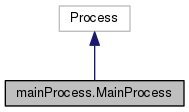
\includegraphics[width=214pt]{classmain_process_1_1_main_process__inherit__graph}
\end{center}
\end{figure}


Collaboration diagram for main\-Process.\-Main\-Process\-:
\nopagebreak
\begin{figure}[H]
\begin{center}
\leavevmode
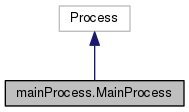
\includegraphics[width=214pt]{classmain_process_1_1_main_process__coll__graph}
\end{center}
\end{figure}
\subsubsection*{Public Member Functions}
\begin{DoxyCompactItemize}
\item 
def \hyperlink{classmain_process_1_1_main_process_a96179f150cf7b4763bb7ea705036efe3}{\-\_\-\-\_\-init\-\_\-\-\_\-}
\begin{DoxyCompactList}\small\item\em Constructor. \end{DoxyCompactList}\item 
def \hyperlink{classmain_process_1_1_main_process_a05fa1ffb2d1357bdaf2cdfb4fedc5d5d}{detect\-Imu}
\begin{DoxyCompactList}\small\item\em Detectes the number of I\-M\-Us avaliable in each channel. \end{DoxyCompactList}\item 
\hypertarget{classmain_process_1_1_main_process_abee13c2eebb46c3990ed9e00e8bab243}{def {\bfseries set\-Poll\-Interval}}\label{classmain_process_1_1_main_process_abee13c2eebb46c3990ed9e00e8bab243}

\item 
def \hyperlink{classmain_process_1_1_main_process_afffc3c5095b0abab4a7c74ceb5b92fa5}{set\-File\-Name}
\begin{DoxyCompactList}\small\item\em Sets file name for the C\-S\-V file. \end{DoxyCompactList}\item 
def \hyperlink{classmain_process_1_1_main_process_ab0a345554ba8ce59d396418fc9b97121}{get\-Data}
\begin{DoxyCompactList}\small\item\em gets the current data from the current sensor \end{DoxyCompactList}\item 
def \hyperlink{classmain_process_1_1_main_process_ab0d698817a4f92499affb3742b14c03a}{stop}
\begin{DoxyCompactList}\small\item\em stops the thread and signals to exit \end{DoxyCompactList}\item 
\hypertarget{classmain_process_1_1_main_process_abf1f1b3f0452593e8e5880d9c881db84}{def {\bfseries save\-Settings}}\label{classmain_process_1_1_main_process_abf1f1b3f0452593e8e5880d9c881db84}

\item 
def \hyperlink{classmain_process_1_1_main_process_a83337e0c06f5fa02705bf309537c8702}{run}
\begin{DoxyCompactList}\small\item\em Thread loop. \end{DoxyCompactList}\end{DoxyCompactItemize}
\subsubsection*{Public Attributes}
\begin{DoxyCompactItemize}
\item 
\hypertarget{classmain_process_1_1_main_process_af4319aca7fa44df660d800c70bab9745}{{\bfseries exit}}\label{classmain_process_1_1_main_process_af4319aca7fa44df660d800c70bab9745}

\item 
\hypertarget{classmain_process_1_1_main_process_a07364aa44c1f097f11e222a8d504ee83}{{\bfseries csv}}\label{classmain_process_1_1_main_process_a07364aa44c1f097f11e222a8d504ee83}

\item 
\hypertarget{classmain_process_1_1_main_process_a9e8c76f292f1deed175b69f9c81091a4}{{\bfseries i2c\-Mux}}\label{classmain_process_1_1_main_process_a9e8c76f292f1deed175b69f9c81091a4}

\item 
\hypertarget{classmain_process_1_1_main_process_a6d5f3226edd5542e1a343930a005a9d9}{{\bfseries settings0}}\label{classmain_process_1_1_main_process_a6d5f3226edd5542e1a343930a005a9d9}

\item 
\hypertarget{classmain_process_1_1_main_process_a483b3165f6cd2a685a84b9eb8fe20fde}{{\bfseries settings1}}\label{classmain_process_1_1_main_process_a483b3165f6cd2a685a84b9eb8fe20fde}

\item 
\hypertarget{classmain_process_1_1_main_process_ae9eae743905bf704b3511658e9b6c3fb}{{\bfseries settings2}}\label{classmain_process_1_1_main_process_ae9eae743905bf704b3511658e9b6c3fb}

\item 
\hypertarget{classmain_process_1_1_main_process_a300e5b3481d6462bad3fb9636ce2de8b}{{\bfseries settings3}}\label{classmain_process_1_1_main_process_a300e5b3481d6462bad3fb9636ce2de8b}

\item 
\hypertarget{classmain_process_1_1_main_process_a31420d2d562bffd08df9ac2c2e8e0882}{{\bfseries settings4}}\label{classmain_process_1_1_main_process_a31420d2d562bffd08df9ac2c2e8e0882}

\item 
\hypertarget{classmain_process_1_1_main_process_a0389ffbb6bc904a950c8363fe641820b}{{\bfseries settings5}}\label{classmain_process_1_1_main_process_a0389ffbb6bc904a950c8363fe641820b}

\item 
\hypertarget{classmain_process_1_1_main_process_a47d56281a5da4a79c08161c681df0d23}{{\bfseries imu0}}\label{classmain_process_1_1_main_process_a47d56281a5da4a79c08161c681df0d23}

\item 
\hypertarget{classmain_process_1_1_main_process_a7f32b196ddbb4b120494bdcc43fac75e}{{\bfseries imu1}}\label{classmain_process_1_1_main_process_a7f32b196ddbb4b120494bdcc43fac75e}

\item 
\hypertarget{classmain_process_1_1_main_process_ac3649d6ca19cfaa8bb9f0cbd97efb4ae}{{\bfseries imu2}}\label{classmain_process_1_1_main_process_ac3649d6ca19cfaa8bb9f0cbd97efb4ae}

\item 
\hypertarget{classmain_process_1_1_main_process_aeaead89db3a8996457e29bc55646a9a9}{{\bfseries imu3}}\label{classmain_process_1_1_main_process_aeaead89db3a8996457e29bc55646a9a9}

\item 
\hypertarget{classmain_process_1_1_main_process_a74889e9e742c2f9c74922e8437d9a400}{{\bfseries imu4}}\label{classmain_process_1_1_main_process_a74889e9e742c2f9c74922e8437d9a400}

\item 
\hypertarget{classmain_process_1_1_main_process_a15c2eb4ca85623b02a243ef5128a2a1b}{{\bfseries imu5}}\label{classmain_process_1_1_main_process_a15c2eb4ca85623b02a243ef5128a2a1b}

\item 
\hypertarget{classmain_process_1_1_main_process_ae194e857c91b74cefe7676fe1310fc55}{{\bfseries settings}}\label{classmain_process_1_1_main_process_ae194e857c91b74cefe7676fe1310fc55}

\item 
\hypertarget{classmain_process_1_1_main_process_a71a330454de16c8e8d1a0ddd1d723f5a}{{\bfseries imus}}\label{classmain_process_1_1_main_process_a71a330454de16c8e8d1a0ddd1d723f5a}

\item 
\hypertarget{classmain_process_1_1_main_process_a91686836c3bff8156c60b6376d76be22}{{\bfseries detected\-I\-M\-U}}\label{classmain_process_1_1_main_process_a91686836c3bff8156c60b6376d76be22}

\item 
\hypertarget{classmain_process_1_1_main_process_a97b9d0f1c87a257cb375c5dce89b3562}{{\bfseries poll\-Interval}}\label{classmain_process_1_1_main_process_a97b9d0f1c87a257cb375c5dce89b3562}

\item 
\hypertarget{classmain_process_1_1_main_process_aefce877b1e08d31b00753b0107e536d8}{{\bfseries all\-Data}}\label{classmain_process_1_1_main_process_aefce877b1e08d31b00753b0107e536d8}

\end{DoxyCompactItemize}


\subsubsection{Detailed Description}
Thread for adquiring data from I\-M\-Us. 


\begin{DoxyParams}{Parameters}
{\em Process} & the process object \\
\hline
\end{DoxyParams}


\subsubsection{Constructor \& Destructor Documentation}
\hypertarget{classmain_process_1_1_main_process_a96179f150cf7b4763bb7ea705036efe3}{\index{main\-Process\-::\-Main\-Process@{main\-Process\-::\-Main\-Process}!\-\_\-\-\_\-init\-\_\-\-\_\-@{\-\_\-\-\_\-init\-\_\-\-\_\-}}
\index{\-\_\-\-\_\-init\-\_\-\-\_\-@{\-\_\-\-\_\-init\-\_\-\-\_\-}!mainProcess::MainProcess@{main\-Process\-::\-Main\-Process}}
\paragraph[{\-\_\-\-\_\-init\-\_\-\-\_\-}]{\setlength{\rightskip}{0pt plus 5cm}def main\-Process.\-Main\-Process.\-\_\-\-\_\-init\-\_\-\-\_\- (
\begin{DoxyParamCaption}
\item[{}]{self}
\end{DoxyParamCaption}
)}}\label{classmain_process_1_1_main_process_a96179f150cf7b4763bb7ea705036efe3}


Constructor. 

Inits the process, the C\-S\-V file, the P\-C\-A9547 Multiplexor, the settings file for each sensor (with calibration) 
\begin{DoxyParams}{Parameters}
{\em self} & The object pointer \\
\hline
\end{DoxyParams}


\subsubsection{Member Function Documentation}
\hypertarget{classmain_process_1_1_main_process_a05fa1ffb2d1357bdaf2cdfb4fedc5d5d}{\index{main\-Process\-::\-Main\-Process@{main\-Process\-::\-Main\-Process}!detect\-Imu@{detect\-Imu}}
\index{detect\-Imu@{detect\-Imu}!mainProcess::MainProcess@{main\-Process\-::\-Main\-Process}}
\paragraph[{detect\-Imu}]{\setlength{\rightskip}{0pt plus 5cm}def main\-Process.\-Main\-Process.\-detect\-Imu (
\begin{DoxyParamCaption}
\item[{}]{self}
\end{DoxyParamCaption}
)}}\label{classmain_process_1_1_main_process_a05fa1ffb2d1357bdaf2cdfb4fedc5d5d}


Detectes the number of I\-M\-Us avaliable in each channel. 


\begin{DoxyParams}{Parameters}
{\em self} & The object pointer \\
\hline
\end{DoxyParams}
\begin{DoxyReturn}{Returns}
number of detected I\-M\-Us 
\end{DoxyReturn}
\hypertarget{classmain_process_1_1_main_process_ab0a345554ba8ce59d396418fc9b97121}{\index{main\-Process\-::\-Main\-Process@{main\-Process\-::\-Main\-Process}!get\-Data@{get\-Data}}
\index{get\-Data@{get\-Data}!mainProcess::MainProcess@{main\-Process\-::\-Main\-Process}}
\paragraph[{get\-Data}]{\setlength{\rightskip}{0pt plus 5cm}def main\-Process.\-Main\-Process.\-get\-Data (
\begin{DoxyParamCaption}
\item[{}]{self}
\end{DoxyParamCaption}
)}}\label{classmain_process_1_1_main_process_ab0a345554ba8ce59d396418fc9b97121}


gets the current data from the current sensor 


\begin{DoxyParams}{Parameters}
{\em self} & The object pointer \\
\hline
\end{DoxyParams}
\begin{DoxyReturn}{Returns}
all sensor data as a vector 
\end{DoxyReturn}
\hypertarget{classmain_process_1_1_main_process_a83337e0c06f5fa02705bf309537c8702}{\index{main\-Process\-::\-Main\-Process@{main\-Process\-::\-Main\-Process}!run@{run}}
\index{run@{run}!mainProcess::MainProcess@{main\-Process\-::\-Main\-Process}}
\paragraph[{run}]{\setlength{\rightskip}{0pt plus 5cm}def main\-Process.\-Main\-Process.\-run (
\begin{DoxyParamCaption}
\item[{}]{self}
\end{DoxyParamCaption}
)}}\label{classmain_process_1_1_main_process_a83337e0c06f5fa02705bf309537c8702}


Thread loop. 

Get data in the polling interval definid time, and stores data form all the avaliable sensor with his identificator and timestamp 
\begin{DoxyParams}{Parameters}
{\em self} & The object pointer \\
\hline
\end{DoxyParams}
\begin{DoxyReturn}{Returns}
finalized job 
\end{DoxyReturn}
\hypertarget{classmain_process_1_1_main_process_afffc3c5095b0abab4a7c74ceb5b92fa5}{\index{main\-Process\-::\-Main\-Process@{main\-Process\-::\-Main\-Process}!set\-File\-Name@{set\-File\-Name}}
\index{set\-File\-Name@{set\-File\-Name}!mainProcess::MainProcess@{main\-Process\-::\-Main\-Process}}
\paragraph[{set\-File\-Name}]{\setlength{\rightskip}{0pt plus 5cm}def main\-Process.\-Main\-Process.\-set\-File\-Name (
\begin{DoxyParamCaption}
\item[{}]{self, }
\item[{}]{txt}
\end{DoxyParamCaption}
)}}\label{classmain_process_1_1_main_process_afffc3c5095b0abab4a7c74ceb5b92fa5}


Sets file name for the C\-S\-V file. 


\begin{DoxyParams}{Parameters}
{\em self} & The object pointer \\
\hline
{\em txt} & file name \\
\hline
\end{DoxyParams}
\hypertarget{classmain_process_1_1_main_process_ab0d698817a4f92499affb3742b14c03a}{\index{main\-Process\-::\-Main\-Process@{main\-Process\-::\-Main\-Process}!stop@{stop}}
\index{stop@{stop}!mainProcess::MainProcess@{main\-Process\-::\-Main\-Process}}
\paragraph[{stop}]{\setlength{\rightskip}{0pt plus 5cm}def main\-Process.\-Main\-Process.\-stop (
\begin{DoxyParamCaption}
\item[{}]{self}
\end{DoxyParamCaption}
)}}\label{classmain_process_1_1_main_process_ab0d698817a4f92499affb3742b14c03a}


stops the thread and signals to exit 


\begin{DoxyParams}{Parameters}
{\em self} & The object pointer \\
\hline
\end{DoxyParams}


The documentation for this class was generated from the following file\-:\begin{DoxyCompactItemize}
\item 
www/main\-Process.\-py\end{DoxyCompactItemize}

\hypertarget{classpca9547_1_1_p_c_a9547}{\subsection{pca9547.\-P\-C\-A9547 Class Reference}
\label{classpca9547_1_1_p_c_a9547}\index{pca9547.\-P\-C\-A9547@{pca9547.\-P\-C\-A9547}}
}


Class to manage the I2\-C Multiplexor \hyperlink{classpca9547_1_1_p_c_a9547}{P\-C\-A9547}.  


\subsubsection*{Public Member Functions}
\begin{DoxyCompactItemize}
\item 
def \hyperlink{classpca9547_1_1_p_c_a9547_a23b8693ebee5b2f8581b43843380de17}{\-\_\-\-\_\-init\-\_\-\-\_\-}
\begin{DoxyCompactList}\small\item\em Consructor. \end{DoxyCompactList}\item 
def \hyperlink{classpca9547_1_1_p_c_a9547_a5b8751a7eed5e81d8ba18b16bbcacbe0}{set\-Channel}
\begin{DoxyCompactList}\small\item\em Sets the current enabled channel. \end{DoxyCompactList}\item 
def \hyperlink{classpca9547_1_1_p_c_a9547_a86abcdfca17635d3aa4e7d2ce44f18d8}{get\-Channel}
\begin{DoxyCompactList}\small\item\em Gets the current enabled channel. \end{DoxyCompactList}\item 
def \hyperlink{classpca9547_1_1_p_c_a9547_a89f0831e00c136b4dc7c58c600f7794e}{reset\-Channel}
\begin{DoxyCompactList}\small\item\em Resets the multiplexor. \end{DoxyCompactList}\end{DoxyCompactItemize}
\subsubsection*{Static Public Attributes}
\begin{DoxyCompactItemize}
\item 
\hypertarget{classpca9547_1_1_p_c_a9547_a4f970ca67e4a1048f6c4c34c723c2452}{\hyperlink{classpca9547_1_1_p_c_a9547_a4f970ca67e4a1048f6c4c34c723c2452}{address} = None}\label{classpca9547_1_1_p_c_a9547_a4f970ca67e4a1048f6c4c34c723c2452}

\begin{DoxyCompactList}\small\item\em Addres of the multiplexor. \end{DoxyCompactList}\end{DoxyCompactItemize}


\subsubsection{Detailed Description}
Class to manage the I2\-C Multiplexor \hyperlink{classpca9547_1_1_p_c_a9547}{P\-C\-A9547}. 



\subsubsection{Constructor \& Destructor Documentation}
\hypertarget{classpca9547_1_1_p_c_a9547_a23b8693ebee5b2f8581b43843380de17}{\index{pca9547\-::\-P\-C\-A9547@{pca9547\-::\-P\-C\-A9547}!\-\_\-\-\_\-init\-\_\-\-\_\-@{\-\_\-\-\_\-init\-\_\-\-\_\-}}
\index{\-\_\-\-\_\-init\-\_\-\-\_\-@{\-\_\-\-\_\-init\-\_\-\-\_\-}!pca9547::PCA9547@{pca9547\-::\-P\-C\-A9547}}
\paragraph[{\-\_\-\-\_\-init\-\_\-\-\_\-}]{\setlength{\rightskip}{0pt plus 5cm}def pca9547.\-P\-C\-A9547.\-\_\-\-\_\-init\-\_\-\-\_\- (
\begin{DoxyParamCaption}
\item[{}]{self, }
\item[{}]{address = {\ttfamily 0x70}}
\end{DoxyParamCaption}
)}}\label{classpca9547_1_1_p_c_a9547_a23b8693ebee5b2f8581b43843380de17}


Consructor. 

Defines the address for the multiplexor 
\begin{DoxyParams}{Parameters}
{\em self} & The objetc pointer \\
\hline
{\em address} & Address to be used \\
\hline
\end{DoxyParams}


\subsubsection{Member Function Documentation}
\hypertarget{classpca9547_1_1_p_c_a9547_a86abcdfca17635d3aa4e7d2ce44f18d8}{\index{pca9547\-::\-P\-C\-A9547@{pca9547\-::\-P\-C\-A9547}!get\-Channel@{get\-Channel}}
\index{get\-Channel@{get\-Channel}!pca9547::PCA9547@{pca9547\-::\-P\-C\-A9547}}
\paragraph[{get\-Channel}]{\setlength{\rightskip}{0pt plus 5cm}def pca9547.\-P\-C\-A9547.\-get\-Channel (
\begin{DoxyParamCaption}
\item[{}]{self}
\end{DoxyParamCaption}
)}}\label{classpca9547_1_1_p_c_a9547_a86abcdfca17635d3aa4e7d2ce44f18d8}


Gets the current enabled channel. 


\begin{DoxyParams}{Parameters}
{\em self} & The objetc pointer \\
\hline
\end{DoxyParams}
\begin{DoxyReturn}{Returns}
the enabled channel number 
\end{DoxyReturn}
\hypertarget{classpca9547_1_1_p_c_a9547_a89f0831e00c136b4dc7c58c600f7794e}{\index{pca9547\-::\-P\-C\-A9547@{pca9547\-::\-P\-C\-A9547}!reset\-Channel@{reset\-Channel}}
\index{reset\-Channel@{reset\-Channel}!pca9547::PCA9547@{pca9547\-::\-P\-C\-A9547}}
\paragraph[{reset\-Channel}]{\setlength{\rightskip}{0pt plus 5cm}def pca9547.\-P\-C\-A9547.\-reset\-Channel (
\begin{DoxyParamCaption}
\item[{}]{self}
\end{DoxyParamCaption}
)}}\label{classpca9547_1_1_p_c_a9547_a89f0831e00c136b4dc7c58c600f7794e}


Resets the multiplexor. 

When reseted, the \hyperlink{classpca9547_1_1_p_c_a9547}{P\-C\-A9547} restore to the default channel, 0. 
\begin{DoxyParams}{Parameters}
{\em self} & The objetc pointer \\
\hline
\end{DoxyParams}
\hypertarget{classpca9547_1_1_p_c_a9547_a5b8751a7eed5e81d8ba18b16bbcacbe0}{\index{pca9547\-::\-P\-C\-A9547@{pca9547\-::\-P\-C\-A9547}!set\-Channel@{set\-Channel}}
\index{set\-Channel@{set\-Channel}!pca9547::PCA9547@{pca9547\-::\-P\-C\-A9547}}
\paragraph[{set\-Channel}]{\setlength{\rightskip}{0pt plus 5cm}def pca9547.\-P\-C\-A9547.\-set\-Channel (
\begin{DoxyParamCaption}
\item[{}]{self, }
\item[{}]{channel = {\ttfamily 0}}
\end{DoxyParamCaption}
)}}\label{classpca9547_1_1_p_c_a9547_a5b8751a7eed5e81d8ba18b16bbcacbe0}


Sets the current enabled channel. 


\begin{DoxyParams}{Parameters}
{\em self} & The objetc pointer \\
\hline
{\em channel} & the channel to enable \\
\hline
\end{DoxyParams}


The documentation for this class was generated from the following file\-:\begin{DoxyCompactItemize}
\item 
www/pca9547.\-py\end{DoxyCompactItemize}

%--- End generated contents ---

% Index
\newpage
\phantomsection
\addcontentsline{toc}{section}{Index}
\printindex

\end{document}
